\chapter{Combat}\label{Combat}
    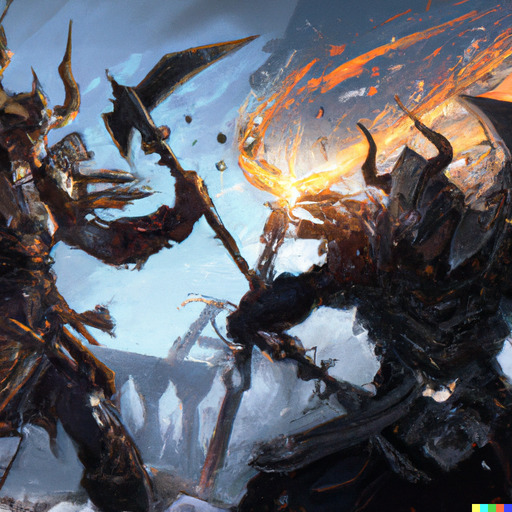
\includegraphics[width=\columnwidth]{combat/combat}
    The world of Rise can be a harsh one, and not all disagreements can be resolved peacefully.
    At some point, you will be forced to enter combat.
    This chapter explains how combat works in Rise.
    The combat rules also generally cover situations where time and precise positioning are important, even if they do not involve violence.

\section{Making Attacks}\label{Attacks}
    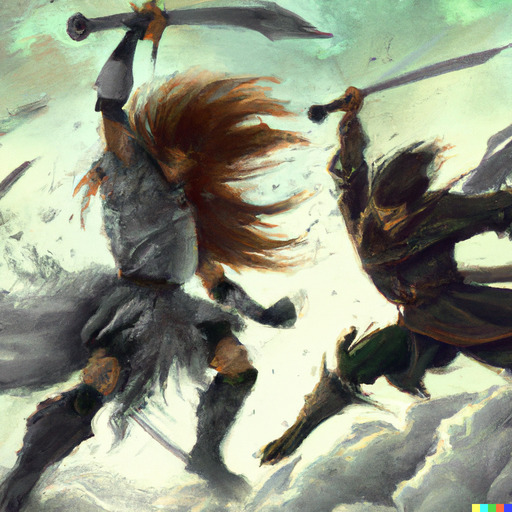
\includegraphics[width=\columnwidth]{core mechanics/making attacks}

    \subsection{Attack Rolls}\label{Attack Rolls}
        To make an attack, roll 1d10 and add your \glossterm{accuracy} with the attack.
        Each attack specifies one or more relevant \glossterm{defenses} which are used to avoid the attack.
        There are four defenses: Armor, Fortitude, Reflex, and Mental.
        Most attacks are made against exactly one defense, which is indicated in the attack's description.

        If the result of your attack roll meets or exceeds the defense of the creature or object you are attacking, the attack hits.
        If your result is 1 or 2 lower than the defender's defense, you get a \glossterm{glancing blow} (see below).
        Otherwise, the attack misses.

        \subsubsection{Glancing Blows}\label{Glancing Blows}
            When you would miss on a damaging attack by 2 or less, you instead get a \glossterm{glancing blow}.
            A glancing blow deals half damage.
            It also does not have any special effects other than immediate damage, unless those effects would also happen on a miss.
            Non-damaging attacks cannot cause glancing blows.

            A glancing blow is neither a hit nor a miss.
            However, some abilities trigger on both glancing blows and missed attacks, such as a \mitem{hardblock shield}.

        \subsubsection{Exploding Attacks}\label{Exploding Attacks}
            When you make an attack roll, if you roll a 10 on the d10, the die \glossterm{explodes}.
            That means you roll it again and add both values to determine your total.
            If you roll a 10 on the extra roll, you keep rolling until it stops exploding and add all of the rolls together.

            The number you need to roll to explode is called your \glossterm{explosion target}.
            It is normally 10, but some effects can reduce your explosion target.
            For example, if your explosion target is reduced by 2, you explode when you roll an 8, 9, or 10.
            Effects which reduce your explosion target do not affect bonus dice rolled for exploding attacks.

        \subsubsection{Critical Hits}\label{Critical Hits}
            If your attack result is at least 10 higher than your target's defense, your attack is a \glossterm{critical hit}.
            Damaging attacks normally deal double damage on a critical hit.
            Some non-damaging attacks also have special effects on a critical hit.

            For every additional increment of 10 by which you beat the target's defense, the effect of a critical hit is repeated, if applicable.
            For example, if you get a double critical with attack that has a critical hit effect of ``The condition must be removed an additional time.'', the condition must be removed two additional times.
            As normal, two doublings become a tripling, so a double critical hit with a damaging attack would roll triple the damage dice.

            The damage multiplier from a critical hit is multiplicative with all other damage modifiers, including attacks that say they deal double damage.
            Typically, you roll damage dice twice for a critical hit and sum both results, along with doubling any flat modifiers.
            If this would require you to roll an inconveniently large number of dice, you can just multiply the result from your normal damage dice instead.

            Objects are not normally subject to critical hits.

    \subsection{Weapon Damage}\label{Weapon Damage}
        Some abilities deal damage based on the weapon you use the ability with.
        Typically, this will simply involve making a \glossterm{strike} (see \pcref{Strikes}).

        Weapon damage dice are defined in the Equipment chapter (see \pcref{Weapons}).
        You gain a bonus to your weapon damage equal to half your \glossterm{power} see (see \pcref{Power}).
        Strikes are typically \glossterm{mundane}, so you would use your \glossterm{mundane power}.
        However, you might use your \glossterm{magical power} instead for \magical strikes.

    \subsection{Extra Damage}\label{Extra Damage}
        Some abilities add \glossterm{extra damage} to your damaging attacks.
        Extra damage generally works in the same way as damage that is inherently part of the attack.
        It is halved on a glancing blow, doubled on critical hits, and so on.

        There are two main differences between extra damage and an attack's base damage.
        First, extra damage is not \glossterm{weapon damage}.
        Second, any individual target of an attack can only take \glossterm{extra damage} once from that attack.

        For example, the \spell{corrosive grasp} spell deals damage immediately, and again during your next action.
        Because both of those damage instances are caused by a single attack roll, extra damage only applies to the first damage instance.
        However, a \spell{wall of fire} would apply extra damage each time a creature passes through it, since a separate attack is made for each instance of damage.

        Most sources of extra damage do not have a specific damage type.
        The extra damage normally has the same damage type as the attack's base damage.
        If extra damage has a specific damage type, it uses that damage type instead of any of the attack's normal damage types.

    \subsection{Weak Strikes}
        Some abilities make weak strikes, which deal less damage than normal strikes.
        When you make a weak strike, you halve flat damage bonuses, such as from your \glossterm{power}.
        Weak strikes do not halve flat damage penalties, such as if you have a negative power.

\section{Taking Damage}\label{Taking Damage}
    Taking damage from attacks reduces your \glossterm{damage resistance}, and then your \glossterm{hit points}, before finally inflicting \glossterm{vital wounds}.
    To calculate your damage resistance and hit points, see \pcref{Combat Statistics}.
    This section explains those concepts in more detail.

    When you are dealt damage, the damage first reduces your \glossterm{damage resistance} (see \pcref{Damage Resistance}).
    Any damage in excess of your remaining damage resistance causes you to lose that many \glossterm{hit points} (see \pcref{Hit Points}).
    Hit points and damage resistance function in the same way, but damage resistance can protect you from debilitating attacks that only work if they make you lose hit points.
    If you are dealt damage that reduces your hit points below 0, you gain one or more \glossterm{vital wounds} (see \pcref{Negative Hit Points}).

    Monsters typically do not gain vital wounds like player characters do.
    Instead, they simply die or fall unconscious when they reach 0 hit points.

    \subsection{Negative Hit Points}\label{Negative Hit Points}
        You can have negative hit points, but only briefly.
        When your hit points drop below 0, you gain a \glossterm{vital wound} (see \pcref{Vital Wounds}).
        You gain an additional vital wound for each increment of your full maximum hit points that you reach in negative hit points.

        If you would regain \glossterm{hit points} while you have negative hit points, you first reset your hit points to 0 before applying the healing.
        In addition, your hit points are reset to 0 at the end of the round if they are still negative.
        This is checked after applying all healing and damage that takes place at the end of the round.
        This also resets the vital wound thresholds that you have suffered, so you will immediately suffer a vital wound if your hit points go negative during the next round.

    \subsection{Damage Types}\label{Damage Types}
        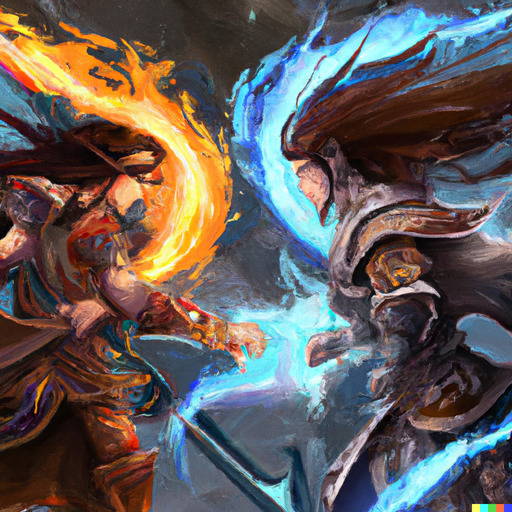
\includegraphics[width=\columnwidth]{core mechanics/damage types}
        There are four main damage types: energy, physical, poison, and psychic.
        Energy and physical damage have additional subtypes, and are much more common than poison or psychic damage.

        \subsubsection{Damage Subtypes}\label{Damage Subtypes}
            Physical damage has four subtypes: acid damage, bludgeoning damage, piercing damage, and slashing damage.
            Energy damage has three subtypes: cold damage, electricity damage, and fire damage.
            Psychic damage has no subtypes.

            Damage of a particular subtype is also considered damage of its primary type.
            For example, if you are \trait{impervious} to \glossterm{physical damage}, that applies against bludgeoning damage because bludgeoning damage is a subtype of \glossterm{physical damage}.

            Some damage types have special properties, as described below.
            \parhead{Cold} Abilities that deal cold damage can freeze liquids and have similar effects appropriate to a sudden drop in temperature.
            \parhead{Electricity} Abilities that deal electricity damage can ignite nonmagical fires if they damage combustible objects.
            \parhead{Fire} Abilities that deal fire damage provide light equivalent to a torch for their duration.
            % TODO: what does this actually mean
            Abilities without a duration create a \glossterm{brief} burst of torchlight.
            While underwater, they deal half damage and have no nondamaging effects.

        \subsubsection{Multiple Damage Types}\label{Multiple Damage Types}
            Some attacks deal damage that has multiple damage types.
            Defensive abilities such as defense bonuses or damage immunities apply against an attack only if they apply to all damage types dealt by the attack.

    \subsection{Special Damage Types}\label{Special Damage Types}

        Subdual damage and environmental damage are separate from the standard damage types, like fire damage or energy damage.
        It is possible for damage to be both environmental damage and subdual damage.

        \subsubsection{Environmental Damage}\label{Environmental Damage}
            Some abilities and environmental effects deal environmental damage.
            Environmental damage is never dealt as the result of a successful attack roll.
            Environmental damage works in the same way as normal damage, except that environmental damage is reduced by your \glossterm{damage resistance} without subtracting from its remaining value.
            Any environmental damage in excess of a creature's damage resistance is causes the creature to lose hit points just like normal damage.

        \subsubsection{Subdual Damage}\label{Subdual Damage}
            Some attacks and environmental effects deal subdual damage.
            Subdual damage works in the same way as normal damage, except it cannot inflict \glossterm{vital wounds}.
            If an attack that deals subdual damage would inflict a vital wound, the target increases its \glossterm{fatigue level} by three instead.
            Whenever you make a \glossterm{strike}, you can choose to deal subdual damage instead of normal damage.
            If you do, you deal half damage with the strike.

\section{Vital Wounds}\label{Vital Wounds}
    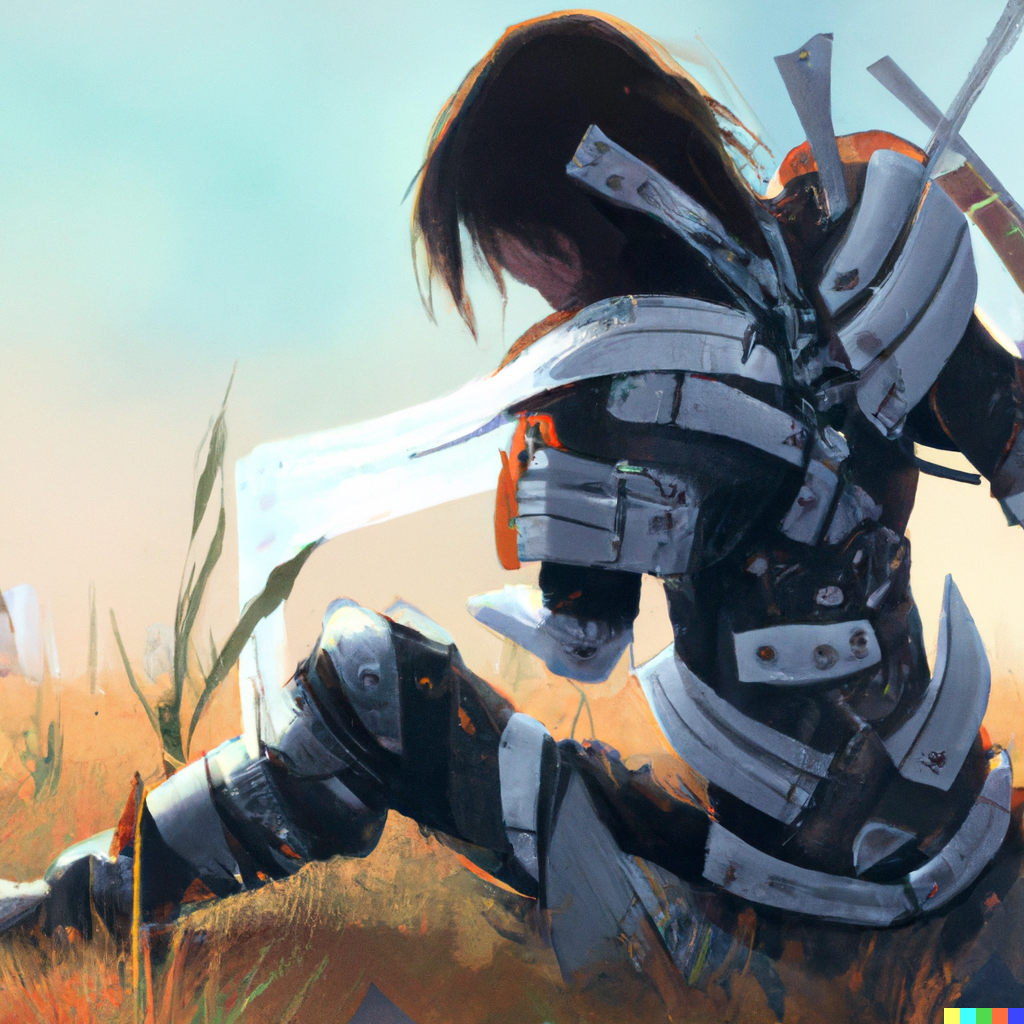
\includegraphics[width=\columnwidth]{core mechanics/vital wounds}

    A \glossterm{vital wound} represents serious damage to your body.
    Each \glossterm{vital wound} has a specific detrimental effect on you.
    You gain vital wounds when your \glossterm{hit points} go negative (see \pcref{Negative Hit Points}).

    To determine the effect of a \glossterm{vital wound}, make a \glossterm{vital roll} and find the corresponding effect in \trefnp{Vital Wound Effects}.
    The effect of the vital wound lasts until you remove that vital wound.
    The effects of vital wounds stack with each other, even if you roll the same effect twice for different \glossterm{vital wounds}.

    \subsection{Vital Rolls}\label{Vital Rolls}
        To make a \glossterm{vital roll}, roll 1d10.
        You take a penalty to this roll equal to twice the number of \glossterm{vital wounds} you already have, not counting the vital wound you are rolling for.
        This includes vital wounds that have no specific vital wound effect.
        The result determines the effect of the \glossterm{vital wound}, as listed in \tref{Vital Wound Effects}.
        Vital wound effects from vital rolls below 1 are lethal if untreated, but the Medicine skill can be used to prevent you from dying (see \pcref{Medicine}).
        This roll is not a \glossterm{check}, so you can't affect it with abilities like \ability{desperate exertion}.

        \begin{dtable}
            \lcaption{Vital Wound Effects}
            \begin{dtabularx}{\textwidth}{l X}
                \tb{Vital Roll}  & \tb{Effect} \tableheaderrule
                \minus6 or less  & You immediately die                                                   \\
                0--\minus5       & You are unconscious, and you die after one minute                     \\
                1                & You are unconscious while you have less than half hit points          \\
                2                & You take a \minus1 penalty to \glossterm{accuracy}                    \\
                3                & You have a \minus5 foot penalty to your speed with all movement modes \\
                4                & Your maximum \glossterm{damage resistance} is halved                  \\
                5                & You take a \minus2 penalty to your \glossterm{fatigue tolerance}      \\
                6                & You take a \minus1 penalty to all \glossterm{defenses}                \\
                7                & You take a \minus2 penalty to your Fortitude defense                  \\
                8                & You take a \minus2 penalty to your Reflex defense                     \\
                9                & You take a \minus2 penalty to your Mental defense                     \\
                10 or more       & No extra vital wound effect                                           \\
            \end{dtabularx}
        \end{dtable}

    \subsection{Removing Vital Wounds}\label{Removing Vital Wounds}
        Vital wounds take time to heal.
        Whenever you finish a \glossterm{long rest}, you remove one of your vital wounds.
        If you have multiple vital wounds, you may choose the order in which your vital wounds are removed.

\section{Combat Time}\label{Combat Time}
    This section explains how time passes in combat.

    \subsection{Rounds}\label{Rounds}

        Combat takes place in a series of \glossterm{rounds}, which represent about six seconds of time.
        Each round of a combat is divided into two \glossterm{phases}: the movement phase and the action phase (see \pcref{Phases}).
        After both phases are complete, the round ends and the next round begins.

    \subsection{Actions}\label{Actions}

        You can take actions in combat to defeat your foes.
        There are three types of actions: \glossterm{standard actions}, \glossterm{minor actions}, and \glossterm{free actions}.
        In addition, you can use \glossterm{movement} during the \glossterm{movement phase} (see \pcref{Movement and Positioning}).
        % TODO: define conflicting action limits (drawing a sword and sheathing a shield?)

        \subsubsection{Standard Actions}\label{Standard Actions}
            Most significant activities require a \glossterm{standard action}.
            This includes attacking with a weapon, casting a \glossterm{spell}, and using many special abilities.
            Using a standard action generally takes about three seconds of time within the game, and it requires most of your attention during that time.

            You can take one standard action during the \glossterm{action phase} of each round.

        \subsubsection{Minor Actions}\label{Minor Actions}
            Some special abilities that take a small amount of time or attention require a \glossterm{minor action}.
            You can take a minor action in the middle of other actions.
            You cannot use a \glossterm{minor action} during the \glossterm{movement phase}.

            You can take one minor action during the \glossterm{action phase} of each round.
            In addition, you can choose to replace your standard action during the action phase with an additional minor action.
            However, you cannot use the same minor action twice in a single round unless an ability specifies otherwise.

        \subsubsection{Free Actions}\label{Free Actions}
            Some activities that take very little time or attention require a \glossterm{free action}.
            You can take a free action in the middle of other actions.

            You can take any number of free actions per round, within reason.
            There is no intrinsic distinction between a free action and something that isn't listed as requiring an action at all.
            However, some free action abilities specify a limit on how often they can be used.
            For example, manipulating objects is a free action, but you can only manipulate an object as a free action once per round (see \pcref{Manipulating Objects}).

    \subsection{Phases}\label{Phases}

        There are two \glossterm{phases} in each round: a \glossterm{movement phase} and an \glossterm{action phase}.
        Each phase specifies the types of actions that can be taken during that phase.
        As a special case, \glossterm{free actions} may be taken during any phase.

        Phases does not represent a specific amount of time.
        In the narrative universe of Rise, movements and actions are intertwined and can happen simultaneously, just as in real life.
        Phases are simply a useful abstraction to keep combat organized.

        \subsubsection{The Movement Phase}\label{The Movement Phase}
            During the \glossterm{movement phase}, you can make one \glossterm{movement}.
            The most common movement is the \textit{hustle} ability, which allows you to move a distance equal to your \glossterm{speed}.
            For details, see \pcref{Movement and Positioning}.

        \subsubsection{The Action Phase}\label{The Action Phase}
            During the \glossterm{action phase}, you can take one \glossterm{minor action} and one \glossterm{standard action}.
            Alternately, you can make a \glossterm{movement} or take an additional \glossterm{minor action} in place of your standard action.
            Most of the time, you will simply take a single standard action.

    \subsection{Resolving Actions}\label{Resolving Actions}

        Actions in combat are partially sequential, and partially simultaneous.
        You and your \glossterm{allies} who can see or otherwise communicate with each other generally act as a single allied group.
        One at a time, each person in the allied group declares their actions, rolls all relevant dice, and applies the results appropriately.
        You can freely choose the order in which people act within the allied group, as long as everyone agrees with the order chosen.
        If one of your allies acts before you, you can learn the result of their action before deciding your own action.
        For example, if they knock an enemy \prone, that enemy would suffer the appropriate defense penalties against your attacks.

        Although your actions resolve sequentially within your allied group, they resolve simultaneously with the actions of anyone outside your allied group.
        Essentially, you locally resolve the effects of your actions within your allied group, but those actions do not globally resolve until later.
        This means that you cannot interrupt enemy actions, even by killing them.
        Generally, you won't know what actions your enemies will take until after you have already resolved your action.
        However, their actions will resolve as if they had acted before you, not after you.
        This goes both ways, of course.
        You can freely decide your actions without knowing what your enemy is doing because their actions cannot interrupt yours.

        Once all allied groups have locally resolved their actions, the results of all of those actions is announced.
        Then, each allied group updates their own status to reflect the actions that all of the other allied groups took during the same phase.
        When resolving these effects, assume that actions outside of your allied group resolve before actions inside of your allied group, as long as they don't alter the effects of your own actions.
        For example, you cannot avoid an enemy attack simply by moving away from them.
        However, an enemy's attack does not interrupt your movement - even if it knocks you unconscious.
        You simply fall unconscious at your new location after the movement.

        Once all of the actions have been globally resolved, the phase ends.
        In a typical combat, this just means that the GM will tell you what the monsters did to you after you tell the GM what you did to them.

        With this system, it's possible for two combatants to kill each other during the same phase, leaving both dead!
        This might seem strange if you're used to other games which always resolve one action at a time.
        However, this situation is not uncommon in fantasty fiction, and it's certainly possible in real life.

        \subsubsection{Delayed and Repeated Effects}
            Some abilities cause additional attacks or effects ``during your next action'' or ``during each of your subsequent actions''.
            Your action happens when you take your turn during the \glossterm{action phase}.
            You can choose when those effects happen during that turn.
            Typically, you would resolve them first so you know their results, but you can do that after your other actions if you want.
            You can't split those automatic effects from your other actions in the turn order, just like you can't take your \glossterm{minor action} separately from your \glossterm{standard action}.

        \subsubsection{Swift Abilities}\label{Swift Abilities}
            Abilities with the \abilitytag{Swift} tag resolve differently from most actions.
            Swift abilities resolve before all non-Swift abilities, so they can change the results of your enemy's actions.
            However, Swift abilities are always simple, and cannot interrupt actions or make attack rolls.
            Generally, they change defenses or recover \glossterm{hit points} or \glossterm{damage resistance}.
            You declare Swift abilities during your normal turn within your allied group, and you don't have to go first within your group or do anything special to use them.

            For example, the \ability{total defense} ability gives you a bonus to your defenses during the current phase.
            That ability has to resolve before your enemies attack you during that phase, or else it would be pointless.
            Some abilities have only part of their effect resolve early.
            For example, the \textit{reckless attack} ability immediately reduces your defenses, which affects attacks made against you during the current phase, and makes a \glossterm{strike} with the normal timing.

        \subsubsection{Action Resolution Summary} 
            \begin{enumerate*}
                \item Round begins - ``start of round'' resolve globally
                \item Movement phase begins - ``start of phase'' effects resolve globally
                \item Movements resolve globally, using \glossterm{initiative} checks when strictly necessary
                \item Movement phase ends - ``end of phase'' effects resolve globally
                \item Action phase begins - ``start of phase'' effects resolve globally
                \item \abilitytag{Swift} abilities resolve globally
                \item Actions of your allied group resolve locally
                \item Actions of other allied groups resolve locally
                \item Actions of each allied group are announced, and resolve globally
                \item Action phase ends - ``end of phase'' effects resolve globally
                \item Round ends - ``end of round'' effects resolve globally
            \end{enumerate*}

        \subsubsection{Deciding Action Order}\label{Deciding Action Order}
            Try not to spend too much time the exact order of everyone's actions within your allied group.
            Most of the time, the exact order doesn't matter.
            It's generally fine to just start rolling dice if you already know what you're going to do, and just act in the order that people decide their actions.
            The GM can help resolve situations where this is ambiguous.

        \subsubsection{Multi-Group Battles}\label{Multi-Group Battles}
            Sometimes, there might be more than two groups in a battle.
            This works in basically the same way as a two-sided battle.
            Each allied group resolves sequentially with itself, but simultaneously with all enemy groups.
            It's possible for two different groups to attack and kill the same creature, which wastes some of their actions.
            That's a natural consequence of not coordinating effectively.

        \subsection{Simultaneous Damage and Healing}\label{Simultaneous Damage and Healing}
            If you regain hit points or damage resistance and take damage simultaneously, apply all damaging effects before applying any healing effects.
            This means you gain and apply the effects of any vital wounds before you are healed.
            Most healing abilities are \abilitytag{Swift}, so this situation should be uncommon.

    \subsection{Conflicting Actions}\label{Conflicting Actions}
        Sometimes, actions that occur in the same phase can be mutually impossible.
        Almost all conflicting actions are the result of competing movements.
        When actions conflict, each creature involved rolls an \glossterm{initiative} check.
        Your initiative modifier is equal to your Dexterity.

        % This may be too complicated?
        Starting from the highest check result and continuing to the lowest, each creature immediately resolves its chosen action.
        Creatures that resolve their action afterward accomplish as much of their intended action as possible before being blocked or otherwise prevented.
        For example, if three different creatures attempt to move into the same space, only the creature with the highest initiative check would actually enter that space.
        The other two creatures would take their intended path, but they would interrupt their movement when they cannot proceed farther, generally because they run into the space occupied by the first creature.

        In general, directly conflicting actions are rare.
        Most movements do not conflict - even reactive movements, such as when one creature attempts to follow a withdrawing creature.
        In that case, no initiative check is necessary.
        Both creatures simply move as far as they can, and the creatures' relative movement speeds determine who is more successful.

        This does make it possible for creatures to be ``stranded'' out of melee range of any attackers.
        Player characters are normally allowed to break this symmetry by reactively using the \textit{sprint} ability, while monsters cannot sprint.
        This can help prevents melee characters from feeling stuck or useless.
        In addition, the \ability{charge} universal ability can be helpful in such cases.

\section{Movement and Positioning}\label{Movement and Positioning}
    This section describes how creatures move and position themselves when time and location are important to measure precisely.

    \subsection{Movements}\label{Movements}
        During each \glossterm{movement phase}, you can make one \glossterm{movement}.
        You can spend your \glossterm{standard action} during the \glossterm{action phase} to make another movement.
        Typically, if you move during the action phase, you would \ability{sprint} to move at double speed (see \pcref{Sprint}).

        When a creature makes a movement, it travels a distance in feet equal to its \glossterm{speed} with one \glossterm{movement mode}.
        Almost all creatures have a land speed, which represents their ability to move across mostly flat terrain.
        For details about other forms of movement, such as flying and swimming, see \pcref{Movement Modes}.

        You can take \glossterm{free actions} and \glossterm{minor actions} in the middle of movement.
        For example, you can walk up to a door, open it, and continue through the door (see \pcref{Manipulating Objects}).

    \subsection{Movement Modes}\label{Movement Modes}
        A \glossterm{movement mode} is a method of moving from one location to another.
        % TODO: terminology confusion mode vs. speed
        The most common movement mode is a land speed, which allows creatures to move across the ground.
        In addition, some abilities grant creatures the ability to move in unusual ways.
        These forms of movement are described here.

        Unless otherwise noted, all creatures have a land speed equal to the base speed for their size (see \pcref{Size Categories}).
        Creatures that are \trait{multipedal} gain a \plus10 foot bonus to their land speed.

        Some creatures have movement modes that are slower than their base speed for various reasons.
        A creature's speed with any given movement mode can never be slower than 5 feet.
        Some effects can still prevent a creature from using their movement modes at all, such as being \immobilized.

        \parhead{Burrowing}
        A creature with a burrow speed can move through the ground at the indicated speed in any direction, even vertically.
        Unless otherwise noted, the creature can only burrow through dirt and loose earth, not rock or harder substances.
        It does not leave behind a usable tunnel for other creatures.

        \parhead{Climbing}
        A creature with a \glossterm{climb speed} can move a distance equal to its climb speed while climbing.
        It must still make a Climb check to move in challenging conditions, such as slippery walls (see \pcref{Climb}).

        \parhead{Flying}
        A creature with a \glossterm{fly speed} can fly through the air at the indicated speed.
        Flying is more complicated than some other movement modes.
        For details, see \pcref{Aerial Movement}.

        \parhead{Gliding}\nonsectionlabel{Gliding}
        A creature with a glide speed can glide through the air at the indicated speed.
        Gliding is more complicated than some other movement modes.
        For details, see \pcref{Aerial Movement}.

        \parhead{Land}
        A creature with a land speed can move across the ground at the indicated speed.

        \parhead{Swimming}
        A creature with a \glossterm{swim speed} can move a distance equal to its swim speed while climbing.
        It must still make a Swim check to move in challenging conditions, such as stormy seas (see \pcref{Swim}).

    \subsection{Combining Movement Modes}
        You can move using multiple different movement modes in the same phase in any order.
        For every 5 feet of speed that you use, you reduce your remaining speed with that movement mode and all movement modes that have an equal or greater remaining speed.

        For example, assume you have a 10 foot climb speed, a 20 foot swim speed, and a 40 foot land speed.
        If you swim 10 feet, you could still climb 10 feet, swim 10 feet, or walk 30 feet as part of the same movement.
        Swimming an additional 10 feet would prevent you from climbing, but you could still walk 20 feet.

    \subsection{Jumping}\label{Jumping}
        Creatures with legs can jump as part of movement.
        When you jump, choose a destination square where your jump ends.
        Landing at a precise location within a square may require a check with the Jump skill (see \pcref{Jump}).

        % Human with 0 strength jumps 5 feet.
        % Human with 2 strength jumps 15 feet.
        % Human with 4 strength jumps 25 feet, which is almost a world record.
        A jump's maximum horizontal distance is normally equal to 5 feet per 2 Strength.
        If you are trained with the Jump skill, the distance is instead equal to 5 feet per Strength, to a minimum of 5 feet.
        If you have a running start of at least 15 feet, you also add a quarter of your \glossterm{base speed} to that distance.
        A jump's maximum vertical height is equal to half your maximum horizontal distance.

        You must be touching a solid surface to jump.
        Jumping off of terrain that is not solid ground, such as a wall, halves your jump distance and may require a Jump check (see \pcref{Jump}).
        If your jump distance would be less than 5 feet, you normally cannot jump meaningfully at all.
        The GM can decide whether that makes sense in a particular situation.

        If your destination square is in midair, you do not start falling until the next phase (see \pcref{Falling Damage}).
        This allows you to jump during the movement phase and act in midair during the action phase.
        Narratively, this represents you timing your jump so you can take a useful action while jumping.
        You don't just hover in midair.

        \subsection{Jumping Speed Limits}
            The maximum distance that you can travel by jumping is equal to your remaining land speed during the current phase.
            This distance is measured only for the farthest extent that you travel from your starting location, not for a round trip or for the entire distance travelled along the arc of your jump.
            For example, if your land speed is thirty feet and you get a ten-foot running start, you can jump no more than twenty feet forward, or fifteen feet forward and five feet vertically, and so on.
            If your jump distance is extremely high and your land speed is low, you may need to use the \ability{sprint} ability to make use of your full jumping potential (see \pcref{Sprint}).

    \subsection{Measuring Movement}

        For simplicity, all movement in combat is measured in five-foot increments.
        While it is possible to be more precise than that, it's generally not worth the complexity.

        \parhead{Squares}\nonsectionlabel{Squares} Area is commonly measured in 5-ft.\ by 5-ft.\ spaces called \glossterm{squares}.
        A single square represents the area occupied by a single humanoid creature in combat.
        Sometimes, movement and distance are represented by the number of squares travelled.
        A 30-ft.\ movement is the same thing as moving six squares.

        \parhead{Diagonals}\nonsectionlabel{Diagonals} When measuring distance, the first diagonal counts as five feet of movement, and the second counds as ten feet of movement.
        The third costs five feet, the fourth costs ten feet, and so on.
        You can move diagonally past corners and enemies.

    \subsection{Movement Abilities}\label{Movement Abilities}

        Almost all creatures can use these abilities to move around a battlefield.
        Many movement abilities are reactive, allowing you to move automatically in response to the movement of other creatures.
        For example, you can try to follow a creature wherever it goes that round.
        In all cases, if you run out of movement speed before accomplishing your intended task, you simply stop where you ran out of movement.

        The most common types of reactive movements are the \textit{block}, \textit{follow}, and \textit{withdraw} abilities, which are described below.
        However, you can can come up with other reactive movements.
        The main requirement is that a reactive movement must have a simple criteria for determining how you move based on easily observable events.
        Secondarily, reactive movements should be simple to resolve.
        If you find yourself rolling a lot of initiative checks to get through the movement phase, you're probably trying to make overly complicated movements.

        \parhead{Hustle}\nonsectionlabel{Hustle} As a \glossterm{movement}, you can use the \textit{hustle} ability to move.
        This is the most common movement ability.

        \begin{activeability}{Hustle}
                \abilityusagetime Standard action.
            \rankline
            Choose a path that you want to travel.
            You travel that path, up to the limit of your relevant movement speed.
        \end{activeability}

        \parhead{Block}\nonsectionlabel{Block} As a \glossterm{movement}, you can use the \textit{block} ability to prevent a creature from entering a particular area.

        \begin{activeability}{Block}[\abilitytag{Swift}]
            \abilityusagetime Standard action.
            \rankline
            When you use this ability, choose a creature you can see.
            During the current phase, whenever that creature attempts to move from a space adjacent to you into another space adjacent to you, you can attempt to block its movement.
            This includes a creature whose path takes it through two consecutive spaces adjacent to you, even if neither the creature's location at the start of the phase nor its intended location at the end of the phase are adjacent to you.
            When you do, make an opposed \glossterm{initiative} check against the target.
            If you beat it on the initiative check, it must spend additional movement equal to one of your relevant movement speeds to move from its space.
            If it cannot, it stops moving.
            This represents you automatically repositioning yourself to block its movement.

            If a creature has the ability to move through your space, such as if it uses the \ability{overrun} ability, it can ignore this additional movement cost.
            If multiple creatures are able to block the same creature from moving, it must pay both additional movement costs, which generally keeps it stuck in place.
        \end{activeability}

        \parhead{Follow}\nonsectionlabel{Follow} As a \glossterm{movement}, you can use the \textit{follow} ability to follow a creature as it moves.

        \begin{activeability}{Follow}
            \abilityusagetime Standard action.
            \rankline
            Choose a creature you can see, and the maximum distance you want to follow at.
            During the current phase, you automatically move such that your distance to the target is no greater than your desired follow distance, up to the limit of your relevant movement speed.

            If the target uses an ability that makes it impossible for you to follow its movement, such as teleporting or disappearing from your sight, it is harder for you to follow its movement.
            If you can see its destination, such as if it teleported to a different location within your \glossterm{line of sight}, you must beat the target on an opposed \glossterm{initiative} check.
            Success means that you can follow its movement normally.
            If you fail at the initiative check, or if you cannot tell where the target went, you complete your movement as if the creature was still at the location where it disappeared.
        \end{activeability}

        \parhead{Withdraw}\nonsectionlabel{Withdraw} As a \glossterm{movement}, you can use the \textit{withdraw} ability to keep away from creatures as they move.

        \begin{activeability}{Withdraw}
            \abilityusagetime Standard action.
            \rankline
            This ability functions like the \textit{follow} ability, except that you specify a minimum distance between you and the target instead of a maximum distance.
            In addition, you can specify multiple targets and try to keep away from all of them.
        \end{activeability}

    \subsection{Movement Impediments}

        \parhead{Difficult Terrain}\nonsectionlabel{Difficult Terrain}
        Some terrain is hard to move through, like thick bushes or a swamp.
        If a square is \glossterm{difficult terrain}, it increases the movement cost required to move out of the square by 5 feet.

        If a square is considered difficult terrain for multiple reasons, the cost increases stack.
        For example, a square in a swamp that also has thick bushes blocking your passage would cost 10 extra feet of movement to leave.

        \parhead{Obstacles}
        An obstacle is anything that gets in your way. Enemies and large solid objects like walls completely block your movement. If you can get past an obstacle, like a low wall, that square is treated as difficult terrain. Some obstacles require a \glossterm{check} to bypass, such as an Balance check (see \pcref{Balance}).

        \parhead{Squeezing}\nonsectionlabel{Squeezing}
        In some cases, you may have to squeeze into or through an area that isn't as wide as the space you take up.
        You can squeeze through or into a space that is at least half as wide as your normal space.
        While \squeezing, you move at half speed, and you take a \minus2 penalty to your Armor and Reflex defenses.
        You can squeeze into tighter spaces with the Flexibility skill.

        Creatures that take up multiple squares take up half their normal number of squares while squeezing. For example, a Large creature who normally takes up four spaces takes up two spaces while squeezing.

        \parhead{Accidentally Squeezing} Sometimes a character ends its movement while moving through a space where it's not normally allowed to stop. When that happens, the character is squeezing in the space until it can move. If squeezing is impossible, the creature immediately moves to the closest available space. Try not to do this.

        \parhead{Undergrowth}\nonsectionlabel{Undergrowth} Vines, roots, bushes, and similar plants that can obstruct sight are common in forested areas.
        These small plants can impede movement in large quantities.
        There are two kinds of undergrowth: \glossterm{light undergrowth} and \glossterm{heavy undergrowth}.

        \subparhead{Light Undergrowth}\nonsectionlabel{Light Undergrowth}
        Light undergrowth provides \glossterm{concealment}.

        \subparhead{Heavy Undergrowth}\nonsectionlabel{Heavy Undergrowth}
        Heavy undergrowth provides \glossterm{concealment} and is \glossterm{difficult terrain}, which increases the movement cost required to move out of each square by 5 feet.

    \subsection{Forced Movement}\label{Forced Movement}
        Some abilities can physically move you against your will.
        Effects that limit movement speed, such as \glossterm{difficult terrain}, similarly limit the distance you can be moved by forced movement effects.
        There are two kinds of forced movement: \glossterm{push} effects and \glossterm{knockback} effects.
        Unless otherwise noted, all forced movement effects move the target in a single straight horizontal line.

        \subsubsection{Push Effects}\label{Push Effects}
            A creature affected by a \glossterm{push} effect is being pushed by a constant force.
            If it encounters another creature or a solid obstacle during the movement, the forced movement effect ends without causing additional harm to the creature or the obstacle.
            Similarly, if a creature being pushed stops being supported and would fall, it falls instead of being pushed further.
            This can allow creatures pushed off the edge of a cliff to grab the edge of the cliff.

        \subsubsection{Knockback Effects}\label{Knockback Effects}
            A creature affected by a \glossterm{knockback} effect is thrown backwards by a single point of impact.
            If it encounters another creature or a solid obstacle during the movement, it and the obstacle each take 1d6 damage per 10 feet of movement remaining.
            A creature moving as a result of a knockback effect does not have to be supported during the movement by solid ground.
            This can allow you to knockback creatures off of cliffs without allowing them to save themselves.

\section{Aerial Movement}\label{Aerial Movement}
    Creatures with a fly speed or glide speed can move in midair to some degree.
    In order to use a fly speed or glide speed, a creature must not be carrying weight in excess of its maximum \glossterm{carrying capacity} (see \pcref{Weight Limits}).
    In addition, it must not have any \glossterm{encumbrance} (see \pcref{Encumbrance}).

    While in midair, land-based creatures cannot move to defend themselves effectively.
    Whenever a creature moves with a fly speed or glide speed, it takes a \minus4 penalty to its Armor and Reflex defenses until it lands on solid ground.
    This penalty does not apply to creatures who are native to the air, such as birds and creatures with no defined land speed.

    A flying or gliding creature must make a \glossterm{movement} using its fly or glide speed during both the \glossterm{movement phase} and the \glossterm{action phase}.
    If it does not move during a phase, it falls by 300 feet at the end of that phase (see \pcref{Falling Damage}).
    \trait{Floating} creatures do not fall in this way.

    \subsection{Gliding}\label{Gliding}
        A creature with a glide speed use a \glossterm{movement} to fall slowly while controlling its direction.
        When it glides, it moves up to its glide speed in any horizontal direction.
        It also must descend 10 feet.
        This descent does not count against its distance moved during the movement.

        In order to glide, a creature must be able to fall.
        Since \trait{floating} creatures cannot fall, they also cannot glide.
        Gliding is impossible in areas without gravity, such as the Astral Plane (see \pcref{Planes}).

    \subsection{Flight}\label{Flight}
        A creature with a fly speed can use a \glossterm{movement} to move up to its fly speed in any direction, even vertically.
        It can also remain in place, though it must still make a \glossterm{movement} each phase to avoid falling.

        \parhead{Height Limit}\nonsectionlabel{Height Limit} Most abilities that grant a fly speed also have a height limit for the maximum height you can reach with that fly speed.
        This height measures your maximum distance above a supporting object.
        The object must be at least two size categories larger than you, and it must be free-standing and capable of supporting your weight.
        It can be up to 5 feet away from you horizontally, which allows you to fly up cliffs and similar structures.
        You can fly above surfaces like water as long as they are thick enough to support your weight.

        While you are above your maximum height with a fly speed, you have a \glossterm{glide speed} equal to your fly speed.

\section{Universal Abilities}\label{Universal Abilities}
    All creatures can use the following abilities.

    \subsection{Strikes}\label{Strikes}
        A \glossterm{strike} is the most common type of attack.
        There are three kinds of strikes: melee, projectile, and thrown.
        Many abilities allow you to make one or more strikes.
        Whenever you make a strike, you can choose which kind of strike to make.

        Your \glossterm{accuracy} with a strike adds the accuracy modifier from the weapon you are attacking with.
        Your \glossterm{damage} with a strike is normally equal to your \glossterm{weapon damage} with the weapon you hit with (see \pcref{Weapon Damage}).

        There are many special rules that can modify how you make strikes.
        For example, \glossterm{dual strikes} allow you to attack with two weapons instead of one.
        The rules for strikes listed here simply define the normal behavior.

        \begin{activeability}*{Basic Strike -- Melee}
            \abilityusagetime Standard action.
            \rankline
            Make an attack vs. Armor using a weapon against anything adjacent to you.
            You must have \glossterm{line of effect} to the target.
            \hit You deal the target \glossterm{weapon damage} from the weapo.
        \end{activeability}

        \begin{activeability}*{Basic Strike -- Projectile}
            \abilityusagetime Standard action.
            \rankline
            Make an attack vs. Armor using a \weapontag{Projectile} weapon against anything that you have \glossterm{line of effect} to.
            If the target is adjacent to you, you take a \minus4 accuracy penalty.
            If the target is at \glossterm{long range} from you, your accuracy takes a \minus4 \glossterm{longshot penalty} (see \pcref{Weapon Range Limits}).
            \hit You deal the target \glossterm{weapon damage} from the weapo.
        \end{activeability}

        \begin{activeability}*{Basic Strike -- Thrown}
            \abilityusagetime Standard action.
            \rankline
            Make an attack vs. Armor using a non-\weapontag{Projectile} weapon against anything that you have \glossterm{line of effect} to.
            If the weapon has the \weapontag{Thrown} weapon tag, use its defined \glossterm{range limits}.
            Otherwise, your range limits are 10/20, and you take a \minus2 accuracy penalty since you are not \glossterm{proficient} with that usage of the weapon (see \pcref{Weapon Proficiency}).
            If the target is at \glossterm{long range} from you, your accuracy takes a \minus4 \glossterm{longshot penalty} (see \pcref{Weapon Range Limits}).
            \hit You deal the target \glossterm{weapon damage} from the weapon.
        \end{activeability}

        \subsubsection{Dual Strikes}\label{Dual Strikes}
            If you are wielding two weapons, you can attack with both at the same time whenever you make a \glossterm{strike}.
            This is called a \glossterm{dual strike}.
            You need a Dexterity of at least 1 to make a dual strike.
            In addition, you cannot use a shield to make dual strikes, even if you are proficient with using it as a weapon.

            When you make a dual strike, you make a separate attack with each weapon.
            Each attack deals its full \glossterm{weapon damage} if it hits.
            You make the attacks sequentially, so you can direct the second attack at a different target depending on the results of the first attack.

            Although a dual strike make two attack rolls, it is still considered to be a single attack.
            Even if you hit a target with both weapons, you still only apply special effects of the attack once.
            This includes \glossterm{extra damage}, any \glossterm{conditions} caused by the strike, and so on.
            Each target hit by either weapon still suffers those full special effects, just like other attacks that can hit multiple targets.

            Dual-wielding has three downsides.
            \begin{itemize}
                \item You cannot get a \glossterm{glancing blow} with either weapon while attacking with two weapons at once (see \pcref{Glancing Blows}).
                    If you would miss by 1 or 2, it is considered a full miss instead of a glancing blow.
                \item You take a \minus1 accuracy penalty with both attacks.
                    If your Dexterity is 4 or higher, this penalty is removed.
                \item For each non-\weapontag{Light} weapon you dual-wield with, you take an additional \minus1 accuracy penalty with both attacks.
                    Each \weapontag{Heavy} weapon instead imposes a \minus2 penalty.
            \end{itemize}

            Some abilities check if you hit or miss with a \glossterm{strike}.
            While dual-wielding, you can both hit and miss with the same strike if you hit with one weapon and miss with the other.

        \subsubsection{Secondary Strike Targets}\label{Secondary Strike Targets}
            Some abilities allow you to make strikes that affect secondary targets in addition to the primary target or targets.
            You make the same attack roll and damage roll against all targets of the strike.
            For example, weapons with the Sweeping weapon tag can make attacks against secondary targets that are close to the primary target.
            If a strike has multiple primary targets, you must choose a single creature to be treated as the primary target for the purpose of all abilities that reference secondary targets.

            Multiple abilities that cause a strike to affect secondary targets stack normally unless noted otherwise.

    \subsection{Special Combat Abilities}\label{Special Combat Abilities}

        This section lists combat abilities that all characters can use.
        Many of these abilities are \abilitytag{Brawling} abilities.
        You use your Strength instead of your Perception to determine your base accuracy with Brawling abilities (see \pcref{Accuracy}).

        \begin{dtable}
            \lcaption{Special Combat Abilities}
            \begin{compresseddtabularx}{\columnwidth}{l X p{6em}}
                \tb{Ability}       & \tb{Brief Description}              & \tb{Tags}                                      \tableheaderrule
                Charge             & Move and attack                     & \tdash                                         \\
                Desperate Exertion & Reroll with a \plus2 bonus          & \tdash                                         \\
                Dirty Trick        & Impose penalty on a foe             & \abilitytag{Size-Based}                        \\
                Escape Grapple     & Stop being grappled                 & \abilitytag{Brawling}                          \\
                Grapple            & Start grappling with a foe          & \abilitytag{Brawling}, \abilitytag{Size-Based} \\
                Maintain Grapple   & Continue grappling with a foe       & \abilitytag{Brawling}, \abilitytag{Swift}      \\
                Overrun            & Move through foe's space            & \abilitytag{Brawling}, \abilitytag{Size-Based} \\
                Recover            & Regain HP and DR, remove conditions & \abilitytag{Swift}                             \\
                Shove              & Move a foe                          & \abilitytag{Brawling}, \abilitytag{Size-Based} \\
                Sprint             & Move at double speed                & \tdash                                         \\
                Total Defense      & Gain \plus2 to defenses             & \abilitytag{Swift}                             \\
                Throw              & Throw a held object                 & \tdash                                         \\
                Trip               & Trip a foe                          & \abilitytag{Brawling}, \abilitytag{Size-Based} \\
            \end{compresseddtabularx}
        \end{dtable}

        \begin{activeability}*{Charge}
            \abilityusagetime Standard action.
            \rankline
            After you use this ability, you \glossterm{briefly} take a \minus2 penalty to all defenses.
            This ability does not have the \abilitytag{Swift} tag, so it does not affect attacks made against you during the current phase.

            Move up to your speed in a single straight line.
            At the end of your movement, you can make a melee \glossterm{strike} from your new location.
        \end{activeability}

        \begin{activeability}*{Desperate Exertion}
            \abilityusagetime Triggered (see text).
            \par \noindent Cost: Two \glossterm{fatigue levels}.
            \rankline
            You \glossterm{reroll} any \glossterm{attack} or \glossterm{check} you just made and gain a \plus2 bonus.
            You can decide to use this ability after you learn whether the original roll succeeded or failed.
            You can even use it after you learn what the effects of a successful attack or check would be, if that is information you could normally learn if it succeeded.
            However, you must use it before using any other abilities or ending your turn.

            You cannot use this to affect rolls that are not attacks or checks, such as \glossterm{vital rolls}.
            You cannot use this ability multiple times to affect the same roll.
        \end{activeability}

        \begin{activeability}*{Dirty Trick}[\abilitytag{Size-Based}]
            \abilityusagetime Standard action.
            \rankline
            When you use this ability, you must describe the kind of dirty trick you are performing.
            For example, you can pull a creature's pants down, throw sand, or otherwise use your environment to attack.
            The same creature can be affected by multiple dirty tricks, but each must apply a different penalty.

            Make a attack with a free hand against the Reflex defense of one creature you \glossterm{touch}.

            On a hit, the target \glossterm{briefly} suffers a \minus2 penalty to one defense of your choice: Armor, Fortitude, Reflex, or Mental.
            You choose the defense, which must be appropriate for the action you described.
        \end{activeability}

        \begin{activeability}*{Escape Grapple}[\abilitytag{Brawling}]
            \abilityusagetime Standard action.
            \rankline
            Make an attack against any number of creatures that you are grappled by.
            Since this is a \abilitytag{Brawling} ability, you use your Strength instead of your Perception to determine your \glossterm{accuracy}.
            You can also entirely replace your normal accuracy with the Flexibility skill (see \pcref{Flexibility}).

            The defense of each creature is equal to the result of the attack it made with its \textit{maintain grapple} ability, or 0 if it did not use that ability.
            % TODO: awkward wording
            For each target, if you hit that target with this attack, it stops being grappled by you and you stop being grappled by it.
        \end{activeability}

        \begin{activeability}*{Grapple}[\abilitytag{Brawling}, \abilitytag{Size-Based}]
            \abilityusagetime Standard action.
            \rankline
            Make an attack with a free hand against the Fortitude and Reflex defenses of one creature you \glossterm{touch}.
            Since this is a \abilitytag{Brawling} ability, you use your Strength instead of your Perception to determine your \glossterm{accuracy}.

            On a hit against both defenses, you and the target are \grappled by each other.
            For details, see \pcref{Grappling}.
            On a critical hit, you also control the grapple (see \pcref{Controlling a Grapple}).
        \end{activeability}

        \begin{activeability}*{Maintain Grapple}[\abilitytag{Brawling}, \abilitytag{Swift}]
            \abilityusagetime \glossterm{Free action} while you are grappling another creature.
            \rankline
            Make an attack against each creature that you are grappling (see \pcref{Grappling}).
            Since this is a \abilitytag{Brawling} ability, you use your Strength instead of your Perception to determine your \glossterm{accuracy}.
            This attack has no immediate effect.
            The result of this roll determines how difficult it is for a creature to escape the grapple during the current round using the \textit{escape grapple} ability.
            If you do not use this ability while you are in a grapple, then creatures can easily escape the grapple with the \textit{escape grapple} ability.
        \end{activeability}

        \begin{activeability}*{Overrun}[\abilitytag{Brawling}, \abilitytag{Size-Based}]
            \abilityusagetime \glossterm{Movement} or standard action.
            \abilitycost One \glossterm{fatigue level} if used as a movement. No cost when used as a standard action.
            \rankline
            Move up to your movement speed in a straight line.
            You can try to move directly through creatures in your way during this movement.
            Each creature in your way can choose to avoid you, allowing you to pass through its square unhindered.
            If a creature does not attempt to avoid you, you make an attack vs. Fortitude against it.
            Since this is a \abilitytag{Brawling} ability, you use your Strength instead of your Perception to determine your \glossterm{accuracy}.

            If you move into a creature's space with this ability, but you do not move out of it, you and the creature are usually considered \squeezing as long as you continue sharing space (see \pcref{Squeezing}).

            On a hit, you can move through each target's space.
            On a miss, you end your movement immediately.
        \end{activeability}

        \begin{activeability}*{Recover}[\abilitytag{Swift}]
            \abilityusagetime Standard action.
            \rankline
            After you use this ability, you increase your \glossterm{fatigue level} by two, and you cannot use it again until you finish a short rest.

            You remove all \glossterm{conditions} affecting you.
            Then, you regain all of your \glossterm{damage resistance} and half of your total \glossterm{hit points}.
            Because this ability has the \abilitytag{Swift} tag, the removed conditions do not affect you during the current phase.
        \end{activeability}

        \begin{activeability}*{Shove}[\abilitytag{Brawling}, \abilitytag{Size-Based}]
            \abilityusagetime Standard action normally, or \glossterm{movement} while grappling.
            \rankline
            If you are grappling or being grappled by a creature, this ability affects all creatures grappling with you (see \pcref{Grappling}).
            Otherwise, choose one creature adjacent to you.

            Make an attack with a free hand against the Fortitude defense of each target.
            Since this is a \abilitytag{Brawling} ability, you use your Strength instead of your Perception to determine your \glossterm{accuracy}.
            You must be able to \glossterm{touch} each target, but unlike normal for touch abilities, you don't have to beat their Reflex defense.
            If a target is not able to use any of its movement speeds, such as if it is being carried by a flying creature, its defense is treated as 0.

            % Critical hit shove should be equivalent to moving without any limitation.
            % This represents 
            On a hit, you can move up to half your movement speed.
            During this movement, you can \glossterm{push} each target 5 feet for each 5 feet that you move.
            If you push a target so it stops being adjacent to you, you stop being able to push it further.
            On a critical hit, or if the target is at least two size categories smaller than you, your movement speed is not halved.
        \end{activeability}

        \begin{activeability}*{Sprint}
            % It's important that this can only be used with movements
            % to prevent it from being abused with abilities like Shove?
            % Is that clear in the text?
            \abilityusagetime \glossterm{Movement} or standard action.
            \abilitycost One \glossterm{fatigue level} if used as a movement. No cost when used as a standard action.
            \rankline
            You can use this ability in the middle of a phase after noticing that your movement is insufficient to keep up with an enemy's reactive movement (see \pcref{Movement Abilities}).

            You can immediately take another \glossterm{movement}.
            For the duration of that movement, you double your speed with all movement modes.
        \end{activeability}

        \begin{activeability}*{Throw}[\abilitytag{Brawling}]
            \abilityusagetime Standard action.
            % Is this worth the complexity?
            % When you use it as a minor action, your throwing distance is halved, your maximum \glossterm{weight category} is one category lighter than normal, and you cannot make an attack roll to hit with the thrown object.
            \rankline
            You throw an object or creature you hold in at least one hand.
            Your normal throwing distance for an arbitrary object is equal to 15 feet plus 5 feet per 2 Strength.
            If the target's \glossterm{weight category} is equal to the maximum weight category you can lift normally, your throwing distance is halved (see \pcref{Weight Categories}).
            You cannot throw objects too heavy for you to lift normally, even if you can push or drag them.

            In order to throw an unwilling creature, it must already be \grappled by you, and you must make an attack against its Fortitude defense.
            Since this is a \abilitytag{Brawling} ability, you use your Strength instead of your Perception to determine your \glossterm{accuracy}.

            Some objects are much easier or harder to throw than others.
            Weapons with the \weapontag{Thrown} weapon tag can be thrown up to their range limits.
            If an object is easy to throw, such as a small dense sphere, you can throw it up to quadruple your normal throwing distance.
            Likewise, a feather or extremely fragile object may be difficult to throw more than a few feet.
            The GM can provide guidance about throwing unusual objects.

            If you throw the target at a creature or object, you can make an attack roll to hit with it, as the \textit{thrown strike} ability.
            That attack roll is rolled separately from the attack roll to throw an unwilling creature, if any.
        \end{activeability}

        \begin{activeability}*{Total Defense}[\abilitytag{Swift}]
            \abilityusagetime Standard action.
            \rankline
            You gain a \plus2 bonus to your \glossterm{defenses} this round.
            Because this ability has the \abilitytag{Swift} tag, this improves your defenses against attacks made against you during the current round.
        \end{activeability}

        \begin{activeability}*{Trip}[\abilitytag{Brawling}, \abilitytag{Size-Based}]
            \abilityusagetime Standard action.
            \rankline
            Make a melee attack using a free hand or a weapon with the Tripping tag against a creature's Fortitude and Reflex defenses (see \pcref{Weapon Tags}).
            If you attack with a weapon, you add the weapon's accuracy bonus, if any, to the attack.
            However, this is not a \glossterm{strike}, so abilities like the \glossterm{Sweeping} weapon tag have no effect on this attack.

            On a hit, the target becomes \prone.
            In addition, if you made the attack with a Tripping weapon and the attack also beat the target's Armor defense, you deal the target \glossterm{weapon damage} based on your weapon.
            You cannot get a \glossterm{glancing blow} with this attack, and this damage is not doubled if you get a \glossterm{critical hit}.
            This is not a \glossterm{strike}, so abilities that improve your strikes do not affect this ability.
        \end{activeability}

    \subsection{Grappling}\label{Grappling}
        A grappling creature is physically struggling with at least one other creature.
        While grappling, you suffer certain penalties and restrictions, as described below.
        Other than these restrictions, you can act normally.
        \begin{itemize}
            \item One of your hands cannot be used for any purposes other than grappling.
                This prevents humanoid creatures from taking any actions which would require having two free hands, such as attacking with \weapontag{Heavy} weapons.
                Monsters without hands must generally use an appropriate appendage, if possible.
            \item You take a \minus2 penalty to Armor and Reflex defenses.
                This penalty is removed if you control the grapple (see below).
            \item You cannot move unless you \glossterm{push} all creatures grappling you, such as with the \ability{shove} ability (see \pcref{Shove}).
                In addition, you cannot \glossterm{push} a creature grappling with you so it stops being adjacent to you.
                However, you can use the \ability{shove} ability to affect creatures you are grappling with as a \glossterm{movement} instead of as a standard action.
            \item You can use the \ability{escape grapple} and \ability{maintain grapple} abilities to stop or continue grappling (see \pcref{Special Combat Abilities}).
        \end{itemize}

        \subsubsection{Controlling a Grapple}\label{Controlling a Grapple}
            Normally, when you use the \textit{grapple} ability, neither creature controls the grapple.
            If you get a critical hit against every grapple participant, you control the grapple.

            If you control a grapple, you gain two benefits.
            First, you do not take the normal \minus2 penalty to Armor and Reflex defenses for being in a grapple.
            Second, you can escape the grapple as a \glossterm{free action}, without having to use the normal \ability{escape grapple} ability.

            To take control of an existing grapple, you can use the \textit{grapple} ability.
            If you hit against the controlling creature, no creature has control of the grapple.
            On a critical hit against each participant, you gain control of the grapple.

\section{Vision and Light}\label{Vision and Light}
    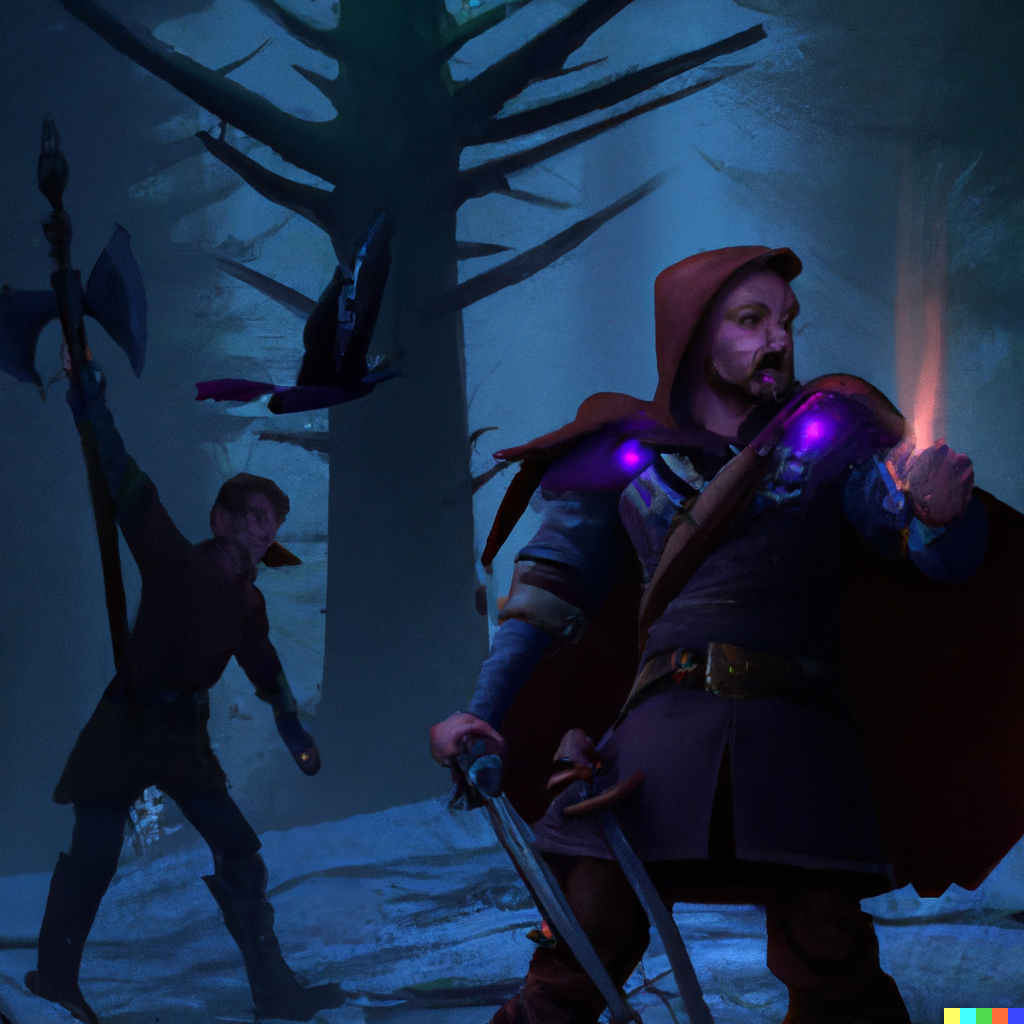
\includegraphics[width=\columnwidth]{combat/vision and light}

    Some creatures have \trait{darkvision} or other extraordinary senses, but most creatures need light to see by. 
    In an area of \glossterm{bright illumination}, all characters can see clearly.

    Creatures can see only dimly into areas that have \glossterm{shadowy illumination}.
    Everything in the area has \glossterm{concealment}.
    This allows creatures in the area to make Stealth checks to hide even if they don't have \glossterm{cover} (see \pcref{Stealth}).

    In an area with \glossterm{brilliant illumination}, creatures can see clearly just like an area with bright illumination.
    In addition, no shadows exist within an an area of brilliant illumination.
    This makes many effects from the \sphere{umbramancy} mystic sphere difficult or impossible to use.

    In areas of total darkness, creatures without \trait{darkvision} or some other form of supernatural vision are \blinded.

    \subsection{Emitting Light}
        Some items and abilities emit light.
        Any effect which creates bright or brilliant illumination in an area also creates enough light for \glossterm{shadowy illumination} in twice that area.

        For example, a simple torch emits \glossterm{bright illumination} in a \smallarea radius.
        That means it also creates \glossterm{shadowy illumination} between 15 feet and 30 feet from the torch in a dark room.

    \subsection{Attacking Unseen Foes}
        You can make \glossterm{targeted} attacks against creatures and objects you cannot see.
        To do so, you choose a 5-foot square and make the attack against that square.
        You have a 50\% \glossterm{miss chance} with the attack.
        Otherwise, you hit a random valid target in that square with your attack, if one exists.

    \subsection{Concealment}\label{Concealment}
        Concealment represents anything which makes it more difficult to see your target, such as \glossterm{shadowy illumination}.
        All \glossterm{targeted} attacks against a creature or object with concealment from you have a 20\% \glossterm{miss chance}.
        Generally, this means that you roll 1d10, and the attack misses on a 1 or 2.
        Determining concealment works similarly to determining cover.
        You must use the same \glossterm{points of origin} and \glossterm{target square} when determining concealment that you would use to determine cover.

        \parhead{Determining Concealment} There are two things that can cause a creature to be concealed: poor lighting, and intervening obstacles that block sight.
        Determining concealment from obstacles that block sight works the same way as determining cover (see \pcref{Cover}).

        Determining concealment from lighting conditions is simpler, since it ignores lighting conditions between you and the target.
        If your \glossterm{target square} is in lighting that provides concealment, the target has concealment.
        Otherwise, it does not.

\section{Obstacles and Cover}\label{Obstacles and Cover}
    In a battle, you may not be able to perfectly see all of your opponents.
    When obstacles get in the way, they may make some attacks impossible.
    Almost all abilities, including \glossterm{strikes}, must have \glossterm{line of sight} and \glossterm{line of effect}.
    Smaller obstacles may simply provide \glossterm{cover} instead of making attacks impossible.
    This section explains how to deal with obstacles and related limitations.

    \subsection{Point of Origin}\label{Point of Origin}
        When you make an attack, you have to determine the \glossterm{point of origin}.
        For \glossterm{targeted} attacks, which are the most common, the point or origin is a grid intersection of your choice that is touching your \glossterm{space}.
        For area attacks, the point of origin depends on the shape of the area and whether it has a defined \glossterm{range}.

        If an area attack has a defined range, the point of origin is a single grid intersection of your choice within that range.
        Cones, lines, and walls without a range use a grid intersection of your choice that is touching your space, just like targeted attacks.
        Cylinders and spheres without a range are unusual, since they radiate from your whole body instead of a single point.
        When determining their total size, treat every grid intersection touching your space as a point of origin.
        When determining cover and similar effects, only use the grid intersection that is closest to the target.

    \subsection{Cover}\label{Cover}

        Cover represents any obstacle that physically prevents you from striking your target, such as a tree or intervening creature.
        A creature or object behind cover gains a \plus2 bonus to Armor and Reflex defenses.
        If an attack would miss or \glossterm{glance} the defense of a creature or object behind cover,
            the attack is instead applied to the obstacle instead of to the intended target.
        In the case of area attacks, this cannot cause an individual creature or object to be targeted or attacked twice by the same ability.
        This can protect creatures behind cover from attacks that deal damage on a miss (see \pcref{Glancing Blows}).
        In addition, a creature behind cover can hide (see \pcref{Stealth}).

        Cover is only relevant if the attacker has \glossterm{line of effect} to its target (see \pcref{Line of Effect}).
        If you don't have line of effect, you generally can't attack the target at all, so the defense bonuses from cover don't matter.

        \subsubsection{Measuring Cover}
            To measure cover for a particular attack, draw a cone from the attack's point of origin to the two closest corners of the target's space.
            For creatures that occupy multiple 5 ft. squares, that these must be corners where the target's space ends, not just grid intersections touching squares the target occupies.
            The defender can choose between equally distant corners.
            If there are any obstacles in that cone, the target has cover.

            Your \glossterm{allies} do not provide cover for attacks you make, as long as you are able to see or hear each other to coordinate.
            In addition, obstacles only provide cover if the relevant part of the obstacle is no more than one size category smaller than the target.
            You should ignore any irrelevant parts of the obstacle that are outside of the cone.
            For example, although a tree might be Gargantuan or Colossal if you include all of its leaves and branches, most trees are only a Medium size obstacle at ground level, since only their trunk is relevant.
            The rules typically ignore the complexity of three-dimensional space, so you'll have to estimate what would provide reasonable cover in some cases.

            \subsubsection{Improved Cover}
            Cover of the same type generally doesn't stack; a creature behind two trees is not substantially more protected than a creature behind a single tree.
            However, exceptionally well covered creatures, such as a creature behind an arrow slit in a castle, may gain a \plus4 benefit to Armor and Reflex defenses rather than the normal \plus2 at the GM's discretion.

    \subsection{Line of Sight}\label{Line of Sight}
        Unless otherwise noted in an ability's description, you cannot target a creature, object, or location that you do not have line of sight to.
        Line of sight measures whether you can see things, not whether you can touch or reach them.

        A line of sight is a straight, unblocked path between an attacker and a target.
        To measure line of sight for a particular attack, draw a line between any grid intersection touching your \glossterm{space} and any grid intersection touching the target's space.
        If you're targeting a particular point, you would naturally draw the line to that point instead.
        If this line is not blocked by any obstacles that impede sight, you have line of sight to your target.

    \subsection{Line of Effect}\label{Line of Effect}
        Almost all abilities, including \glossterm{strikes}, must have a \glossterm{line of effect} to function.
        Line of effect measures whether physical passage is possible between two locations, regardless of any sight obstacles.
        For example, a pane of glass would block line of effect, but not line of sight.

        Unless otherwise noted in an ability's description, you cannot target a creature, object, or location that you do not have line of effect to.
        In addition, abilities that affect an area do not affect targets that the ability does not have line of effect to.

        A line of effect is a straight, unblocked path between an attacker and a target.
        To measure line of sight for a particular attack, draw a line between the attack's \glossterm{point of origin} and any grid intersection touching the target's space.
        If you're targeting a particular point, you would naturally draw the line to that point instead.
        If this line is not blocked by any obstacles that make physical passage impossible, you have line of effect to your target.

        \subsubsection{Destroying Barriers}\label{Destroying Barriers}
            Some abilities deal damage to both creatures and objects.
            If a physical barrier is \glossterm{broken} by an ability, that barrier does not affect the ability's line of effect.
            For example, a thin curtain of silk normally blocks line of effect.
            However, an ability that destroyed the curtain would have its full effect on everything behind the curtain.

        \subsubsection{Inside Creatures}
            Creatures block line of effect to the inside of their own bodies.
            As a result, you cannot use an ability that takes effect inside a creature unless you are also inside the creature.
            This restriction applies even if there is no physical barrier to the inside of the creature.
            For example, you cannot place the \glossterm{point of origin} for an area inside a creature's mouth, even if the creature has its mouth open at the time.

\section{Awareness and Surprise}\label{Awareness and Surprise}
    In combat, creatures are sometimes not fully aware of danger, which makes them less able to defend against it.
    A creature can be described as either aware, \unaware, or \partiallyunaware of an attack against it.
    Normally, creatures are aware of all attacks against them in combat.
    This causes no special bonuses or penalties.

    Sometimes, creatures are fully \unaware that they are in danger from attack.
    This typically happens as a result of stealth, but it can also happen as a result of sudden treachery.
    A creature takes a \minus6 penalty to Armor and Reflex defenses against attacks that it is unaware of.
    After being attacked, an unaware creature typically stops being fully unaware of future attacks.

    A creature that knows that it is in danger and is attempting to defend itself, but does not know the exact location or nature of its attackers, is \partiallyunaware.
    For example, a creature that is already in combat that is attacked by a previously unseen foe is partially unaware of the attack.
    Similarly, a creature that just barely fails to beat an opponent's Stealth check may hear an ominous sound that makes it partially aware of danger without knowing the exact location of any attackers.

    \subsection{Surprise Attacks}\label{Surprise Attacks}
        Sometimes, creatures are not aware that combat is taking place when the combat starts.
        This most commonly happens with ambushes.
        Any creature that is not aware of the combat continues taking whatever actions it would normally be taking until it becomes aware of the combat.
        It is usually \unaware of all until that point, though unusually vigilant or perceptive creatures may be \partiallyunaware.

        If a surprise attack begins a combat, the creatures who initiate the attack can choose which phase to start in.
        Generally, they should start in \glossterm{action phase}, though sometimes the \glossterm{movement phase} is more advantageous for the attackers.

% TODO: This is a bad name; organize these better
\section{Special Combat Rules}

    \subsection{Mounted Combat}\label{Mounted Combat}
        \parhead{Horses in Combat} Warhorses and warponies can serve readily as combat steeds. Light horses, ponies, and heavy horses, however, are frightened by combat.
        At the start of each round, you must make a \glossterm{difficulty value} 10 Ride check to control such a horse.
        Success means you can act normally that round, directing the horse's movements as if it was trained for combat.
        Failure means that the horse acts of its own volition that round, usually fleeing in panic.

        \parhead{Space} A horse (not a pony) is a Large creature, and thus takes up a space 10 feet (2 squares) across. While mounted, you share your mount's space completely. Anyone who is close enough to hit your mount can attack either you or your mount.

        In the case of abnormally large mounts (two or more size categories larger than you), you may not completely share space. Such situations should be handled on a case-by-case basis, depending on the nature of the mount.

        \parhead{Flying Mounts} Flying mounts are harder to ride and control than terrestrial mounts.
        The \glossterm{difficulty value} for all Ride checks on a mount using a fly speed is increased by 10.

        \parhead{Combat while Mounted} With a \glossterm{difficulty value} 5 Ride check, you can guide your mount with your knees so as to use both hands to attack or defend yourself. This is a free action.

        If your mount is moving in the current phase, you take a \minus2 accuracy penalty with ranged strikes.
        If your mount uses the \textit{sprint} ability, this penalty increases to \minus4 (see \pcref{Sprint}).

        \parhead{If Your Mount Falls in Battle} If your mount falls, you fall to the ground with it.

        \parhead{If You Are Dropped} If you are knocked unconscious, you fall from your mount to the ground, which may cause you to take \glossterm{falling damage}.
        If you have a military saddle, you stay on your mount instead.
        In either case, the mount acts according to its nature.
        Most mounts flee combat without a rider.

    \subsection{Allies and Enemies}\label{Allies and Enemies}
        Each creature you interact with in Rise is either an \glossterm{ally}, an \glossterm{enemy}, or neither.
        Some beneficial abilities only affect allies, and some offensive abilities only affect enemies.

        You can choose how you consider each creature at the start of each \glossterm{phase}.
        You cannot consider yourself an \glossterm{ally} or an \glossterm{enemy}.
        While you are \unconscious, you treat all creatures as \glossterm{allies}.

        Some abilities exclusively target allies or enemies, but it might seem appropriate for them to include objects as well in a particular situation.
        The GM can decide whether that makes sense.
        For example, a fighter can normally use the \ability{whirlwind} maneuver to hit all adjacent enemies, and they might want to use that maneuver to destroy a number of objects surrounding them.
        A GM might decide that it's fine to use that maneuver to damage several large objects at once, but the fighter couldn't individually attack fifty specific gold pieces out of a large pile.

        \parhead{Allies} An ally is any creature you consider an ally who also considers you an ally.
        If you consider someone an ally, but they do not consider you an ally, they are not your ally.
        Allies can move through your \glossterm{space}.

        \parhead{Enemies} An enemy is any creature who you consider to be an enemy.
        Enemies cannot move through your \glossterm{space}.

        \parhead{Neutral Parties} A neutral party is any creature who is neither an ally nor an enemy.
        You treat all creatures you have not declared an opinion of as neutral parties.
        Neutral parties can move through your \glossterm{space}.
